\documentclass{ximera}

%\usepackage{todonotes}

\newcommand{\todo}{}

\usepackage{esint} % for \oiint
\ifxake%%https://math.meta.stackexchange.com/questions/9973/how-do-you-render-a-closed-surface-double-integral
\renewcommand{\oiint}{{\large\bigcirc}\kern-1.56em\iint}
\fi


\graphicspath{
  {./}
  {ximeraTutorial/}
  {basicPhilosophy/}
  {functionsOfSeveralVariables/}
  {normalVectors/}
  {lagrangeMultipliers/}
  {vectorFields/}
  {greensTheorem/}
  {shapeOfThingsToCome/}
  {dotProducts/}
  {partialDerivativesAndTheGradientVector/}
  {../productAndQuotientRules/exercises/}
  {../normalVectors/exercisesParametricPlots/}
  {../continuityOfFunctionsOfSeveralVariables/exercises/}
  {../partialDerivativesAndTheGradientVector/exercises/}
  {../directionalDerivativeAndChainRule/exercises/}
  {../commonCoordinates/exercisesCylindricalCoordinates/}
  {../commonCoordinates/exercisesSphericalCoordinates/}
  {../greensTheorem/exercisesCurlAndLineIntegrals/}
  {../greensTheorem/exercisesDivergenceAndLineIntegrals/}
  {../shapeOfThingsToCome/exercisesDivergenceTheorem/}
  {../greensTheorem/}
  {../shapeOfThingsToCome/}
  {../separableDifferentialEquations/exercises/}
  {vectorFields/}
}

\newcommand{\mooculus}{\textsf{\textbf{MOOC}\textnormal{\textsf{ULUS}}}}

\usepackage{tkz-euclide}
\usepackage{tikz}
\usepackage{tikz-cd}
\usetikzlibrary{arrows}
\tikzset{>=stealth,commutative diagrams/.cd,
  arrow style=tikz,diagrams={>=stealth}} %% cool arrow head
\tikzset{shorten <>/.style={ shorten >=#1, shorten <=#1 } } %% allows shorter vectors

\usetikzlibrary{backgrounds} %% for boxes around graphs
\usetikzlibrary{shapes,positioning}  %% Clouds and stars
\usetikzlibrary{matrix} %% for matrix
\usepgfplotslibrary{polar} %% for polar plots
\usepgfplotslibrary{fillbetween} %% to shade area between curves in TikZ
%\usetkzobj{all}
\usepackage[makeroom]{cancel} %% for strike outs
%\usepackage{mathtools} %% for pretty underbrace % Breaks Ximera
%\usepackage{multicol}
\usepackage{pgffor} %% required for integral for loops



%% http://tex.stackexchange.com/questions/66490/drawing-a-tikz-arc-specifying-the-center
%% Draws beach ball
\tikzset{pics/carc/.style args={#1:#2:#3}{code={\draw[pic actions] (#1:#3) arc(#1:#2:#3);}}}



\usepackage{array}
\setlength{\extrarowheight}{+.1cm}
\newdimen\digitwidth
\settowidth\digitwidth{9}
\def\divrule#1#2{
\noalign{\moveright#1\digitwidth
\vbox{\hrule width#2\digitwidth}}}




% \newcommand{\RR}{\mathbb R}
% \newcommand{\R}{\mathbb R}
% \newcommand{\N}{\mathbb N}
% \newcommand{\Z}{\mathbb Z}

\newcommand{\sagemath}{\textsf{SageMath}}


%\renewcommand{\d}{\,d\!}
%\renewcommand{\d}{\mathop{}\!d}
%\newcommand{\dd}[2][]{\frac{\d #1}{\d #2}}
%\newcommand{\pp}[2][]{\frac{\partial #1}{\partial #2}}
% \renewcommand{\l}{\ell}
%\newcommand{\ddx}{\frac{d}{\d x}}

% \newcommand{\zeroOverZero}{\ensuremath{\boldsymbol{\tfrac{0}{0}}}}
%\newcommand{\inftyOverInfty}{\ensuremath{\boldsymbol{\tfrac{\infty}{\infty}}}}
%\newcommand{\zeroOverInfty}{\ensuremath{\boldsymbol{\tfrac{0}{\infty}}}}
%\newcommand{\zeroTimesInfty}{\ensuremath{\small\boldsymbol{0\cdot \infty}}}
%\newcommand{\inftyMinusInfty}{\ensuremath{\small\boldsymbol{\infty - \infty}}}
%\newcommand{\oneToInfty}{\ensuremath{\boldsymbol{1^\infty}}}
%\newcommand{\zeroToZero}{\ensuremath{\boldsymbol{0^0}}}
%\newcommand{\inftyToZero}{\ensuremath{\boldsymbol{\infty^0}}}



% \newcommand{\numOverZero}{\ensuremath{\boldsymbol{\tfrac{\#}{0}}}}
% \newcommand{\dfn}{\textbf}
% \newcommand{\unit}{\,\mathrm}
% \newcommand{\unit}{\mathop{}\!\mathrm}
% \newcommand{\eval}[1]{\bigg[ #1 \bigg]}
% \newcommand{\seq}[1]{\left( #1 \right)}
% \renewcommand{\epsilon}{\varepsilon}
% \renewcommand{\phi}{\varphi}


% \renewcommand{\iff}{\Leftrightarrow}

% \DeclareMathOperator{\arccot}{arccot}
% \DeclareMathOperator{\arcsec}{arcsec}
% \DeclareMathOperator{\arccsc}{arccsc}
% \DeclareMathOperator{\si}{Si}
% \DeclareMathOperator{\scal}{scal}
% \DeclareMathOperator{\sign}{sign}


%% \newcommand{\tightoverset}[2]{% for arrow vec
%%   \mathop{#2}\limits^{\vbox to -.5ex{\kern-0.75ex\hbox{$#1$}\vss}}}
% \newcommand{\arrowvec}[1]{{\overset{\rightharpoonup}{#1}}}
% \renewcommand{\vec}[1]{\arrowvec{\mathbf{#1}}}
% \renewcommand{\vec}[1]{{\overset{\boldsymbol{\rightharpoonup}}{\mathbf{#1}}}}

% \newcommand{\point}[1]{\left(#1\right)} %this allows \vector{ to be changed to \vector{ with a quick find and replace
% \newcommand{\pt}[1]{\mathbf{#1}} %this allows \vec{ to be changed to \vec{ with a quick find and replace
% \newcommand{\Lim}[2]{\lim_{\point{#1} \to \point{#2}}} %Bart, I changed this to point since I want to use it.  It runs through both of the exercise and exerciseE files in limits section, which is why it was in each document to start with.

% \DeclareMathOperator{\proj}{\mathbf{proj}}
% \newcommand{\veci}{{\boldsymbol{\hat{\imath}}}}
% \newcommand{\vecj}{{\boldsymbol{\hat{\jmath}}}}
% \newcommand{\veck}{{\boldsymbol{\hat{k}}}}
% \newcommand{\vecl}{\vec{\boldsymbol{\l}}}
% \newcommand{\uvec}[1]{\mathbf{\hat{#1}}}
% \newcommand{\utan}{\mathbf{\hat{t}}}
% \newcommand{\unormal}{\mathbf{\hat{n}}}
% \newcommand{\ubinormal}{\mathbf{\hat{b}}}

% \newcommand{\dotp}{\bullet}
% \newcommand{\cross}{\boldsymbol\times}
% \newcommand{\grad}{\boldsymbol\nabla}
% \newcommand{\divergence}{\grad\dotp}
% \newcommand{\curl}{\grad\cross}
%\DeclareMathOperator{\divergence}{divergence}
%\DeclareMathOperator{\curl}[1]{\grad\cross #1}
% \newcommand{\lto}{\mathop{\longrightarrow\,}\limits}

% \renewcommand{\bar}{\overline}

\colorlet{textColor}{black}
\colorlet{background}{white}
\colorlet{penColor}{blue!50!black} % Color of a curve in a plot
\colorlet{penColor2}{red!50!black}% Color of a curve in a plot
\colorlet{penColor3}{red!50!blue} % Color of a curve in a plot
\colorlet{penColor4}{green!50!black} % Color of a curve in a plot
\colorlet{penColor5}{orange!80!black} % Color of a curve in a plot
\colorlet{penColor6}{yellow!70!black} % Color of a curve in a plot
\colorlet{fill1}{penColor!20} % Color of fill in a plot
\colorlet{fill2}{penColor2!20} % Color of fill in a plot
\colorlet{fillp}{fill1} % Color of positive area
\colorlet{filln}{penColor2!20} % Color of negative area
\colorlet{fill3}{penColor3!20} % Fill
\colorlet{fill4}{penColor4!20} % Fill
\colorlet{fill5}{penColor5!20} % Fill
\colorlet{gridColor}{gray!50} % Color of grid in a plot

\newcommand{\surfaceColor}{violet}
\newcommand{\surfaceColorTwo}{redyellow}
\newcommand{\sliceColor}{greenyellow}




\pgfmathdeclarefunction{gauss}{2}{% gives gaussian
  \pgfmathparse{1/(#2*sqrt(2*pi))*exp(-((x-#1)^2)/(2*#2^2))}%
}


%%%%%%%%%%%%%
%% Vectors
%%%%%%%%%%%%%

%% Simple horiz vectors
\renewcommand{\vector}[1]{\left\langle #1\right\rangle}


%% %% Complex Horiz Vectors with angle brackets
%% \makeatletter
%% \renewcommand{\vector}[2][ , ]{\left\langle%
%%   \def\nextitem{\def\nextitem{#1}}%
%%   \@for \el:=#2\do{\nextitem\el}\right\rangle%
%% }
%% \makeatother

%% %% Vertical Vectors
%% \def\vector#1{\begin{bmatrix}\vecListA#1,,\end{bmatrix}}
%% \def\vecListA#1,{\if,#1,\else #1\cr \expandafter \vecListA \fi}

%%%%%%%%%%%%%
%% End of vectors
%%%%%%%%%%%%%

%\newcommand{\fullwidth}{}
%\newcommand{\normalwidth}{}



%% makes a snazzy t-chart for evaluating functions
%\newenvironment{tchart}{\rowcolors{2}{}{background!90!textColor}\array}{\endarray}

%%This is to help with formatting on future title pages.
\newenvironment{sectionOutcomes}{}{}



%% Flowchart stuff
%\tikzstyle{startstop} = [rectangle, rounded corners, minimum width=3cm, minimum height=1cm,text centered, draw=black]
%\tikzstyle{question} = [rectangle, minimum width=3cm, minimum height=1cm, text centered, draw=black]
%\tikzstyle{decision} = [trapezium, trapezium left angle=70, trapezium right angle=110, minimum width=3cm, minimum height=1cm, text centered, draw=black]
%\tikzstyle{question} = [rectangle, rounded corners, minimum width=3cm, minimum height=1cm,text centered, draw=black]
%\tikzstyle{process} = [rectangle, minimum width=3cm, minimum height=1cm, text centered, draw=black]
%\tikzstyle{decision} = [trapezium, trapezium left angle=70, trapezium right angle=110, minimum width=3cm, minimum height=1cm, text centered, draw=black]


\title{Quadratic Analysis}

\begin{document}

\begin{abstract}
behavior
\end{abstract}
\maketitle





\section{Quadratic Analysis}

What do we want to know when we analyze any function?

We want to know the 
\begin{itemize}
     \item \textbf{\textcolor{red!80!black}{Domain}} 
     \item \textbf{\textcolor{red!80!black}{Zeros}} 
     \item \textbf{\textcolor{red!80!black}{Continuity}} 
\begin{itemize}
     \item \textbf{\textcolor{red!80!black}{discontinuities}} 
     \item \textbf{\textcolor{red!80!black}{singularities}} 
\end{itemize}
     \item \textbf{\textcolor{red!80!black}{End-Behavior}} 
     \item \textbf{\textcolor{red!80!black}{Behavior}} 
\begin{itemize}
     \item \textbf{\textcolor{red!80!black}{intervals where increasing}} 
     \item \textbf{\textcolor{red!80!black}{intervals where decreasing}} 
\end{itemize}
     \item \textbf{\textcolor{red!80!black}{Global Maximum and Minimum}} 
     \item \textbf{\textcolor{red!80!black}{Local Maximums and Minimums}} 
     \item \textbf{\textcolor{red!80!black}{Range}} 
     \item \textbf{\textcolor{blue!55!black}{...and we would like a nice graph}} 
\end{itemize}

We want all of this information for quadratic functions and we want exact information, not approximations. \\


Quadratic functions are those functions which can be described with formulas like

\begin{itemize}
     \item $A \, x^2 + B \, x + C$
     \item $A \, (x - H)^2 + K$
     \item $A \, (x - r_1) (x-r_2)$
\end{itemize}

For a quadratic function much of the analysis information is connected to vertex of the graph, which is why we like the vertex form, which is why we like completing the square.  But, we can get all of our information from the standard or factored forms as well.





\subsection*{Domain} 

Quadratic functions are defined for all real numbers.  Their natural domain is $\mathbb{R}$. \\

If you can identify a function as quadratic, then you automatically know its domain. \\











\subsection*{Zeros}


The quadratic formula gives the zeros of a quadratic funciton, when we have the \textit{standard form}. The quadratic formula gives the solutions to the quadratic equation

\[
a \, x^2 + b \, x + c = 0
\]

\[ t  =   \frac{-b \pm \sqrt{b^2 - 4 a c}}{2a}      \]



which we can separate into 



\[ t  =   \frac{-b}{2a} \pm \frac{\sqrt{b^2 - 4 a c}}{2a}      \]


The $\pm$ shows that the zeros are symmetric about $\frac{-b}{2a}$ and the intercepts are symmetric about the line $x = \frac{-b}{2a}$. \\

Intercepts are $\left(  \frac{-b - \sqrt{b^2 - 4 a c}}{2a}, 0 \right)$ and $\left(  \frac{-b + \sqrt{b^2 - 4 a c}}{2a}, 0 \right)$.





\begin{image}
\begin{tikzpicture}
     \begin{axis}[
                domain=-10:10, ymax=10, xmax=10, ymin=-10, xmin=-10,
                axis lines =center, xlabel=$x$, ylabel=$y$,
                ytick={-10,-8,-6,-4,-2,2,4,6,8,10},
                xtick={-10,-8,-6,-4,-2,2,4,6,8,10},
                ticklabel style={font=\scriptsize},
                every axis y label/.style={at=(current axis.above origin),anchor=south},
                every axis x label/.style={at=(current axis.right of origin),anchor=west},
                axis on top,
                ]


        \addplot [draw=penColor, very thick, smooth, domain=(1:5),<->] {-2*(x-3)^2 + 4};
        \addplot [line width=1, gray, dashed,samples=100,domain=(-9.5:9.5)] ({3},{x});
        %\addplot [color=penColor2,only marks,mark=*] coordinates{(3,4)};

        \addplot [color=penColor2,only marks,mark=*] coordinates{(1.585,0)};
        \addplot [color=penColor2,only marks,mark=*] coordinates{(4.414,0)};
        


        %\node[penColor] at (axis cs:5,4) {$(h, k))$};
        %\node[penColor] at (axis cs:5,-9) {$-0.5 x^2 - 5 x + 15.5$};



    \end{axis}
\end{tikzpicture}
\end{image}





Working backwards, we can see that if we have the zeros, like from factoring, then we have the intercepts, and the \textbf{line of symmetry} must run in the middle. \\











\subsection*{Continuity}

Quadratic functions are continuous functions.  They have no discontinuities or singularities. \\












\subsection*{End-Behavior}

Quadratic functions have the same end-behavior on both sides, which is given by the sign of the leading coefficient. \\


End-behavior describes what the function is doing out in the ``tails'' of the domain.  That is where the domain numbers are really really really really big positively or negatively. \\

For quadratic functions, $f(x) = a \, x^2 + b x + c$, when $x$ is really really really really big positively or negatively, then the leading term ``dominates'' the other two terms.  The whole function behaves just like $a \, x^2$. \\

That tells us that the whole function will become unbounded. \\


\begin{itemize}
     \item Quadratic functions become unbounded positively if the leading coefficient is positive.
     \item Quadratic functions become unbounded negatively if the leading coefficient is negative.
\end{itemize}



\begin{idea} \textbf{\textcolor{red!80!black}{A Peek Ahead}}

We will want some mathematical notation for end-behavior.  Limit notation will be introduced later and that will be our way of algebraically describing end-behavior. \\

\end{idea}


\begin{example}

Let $g(t) = -2 \, t^2 + 7t - 3$. \\


The end-behavior will be describe as 

\[
$\lim\limits_{t \to -\infty} g(t) = -\infty$
\]


\[
$\lim\limits_{t \to \infty} g(t) = -\infty$
\]

\end{example}








\subsection*{Behavior}



\textbf{\textcolor{blue!55!black}{Increasing and Decreasing}}






The graph vividly suggests that quadratic functions switch from increasing to decreasing (or vice versa) at the symmetric/vertex number in the domain.


\begin{itemize}
\item If the graph is opening up, then the quadratic function is \\

decreasing on $\left( -\infty, \frac{-b}{2a} \right)$ and increasing on $\left( \frac{-b}{2a}, \infty \right)$

\item If the graph is opening down, then the quadratic function is \\

increasing on $\left( -\infty, \frac{-b}{2a} \right)$ and decreasing on $\left( \frac{-b}{2a}, \infty \right)$
\end{itemize}





Increasing and decreasing refer to the rate of change.


\begin{itemize}
\item Increasing is a positive rate of change.
\item Decreasing is a negative rate of change.
\end{itemize}



Now, we can replace our graphical intuition with algebraic rigor. \\ 

We have seen if we write a quadratic function as $f(x) = a (x - h)^2 + k$, then the instantaneous rate of change of $f$ is the linear function $iRoC_f(x) = 2 a (x - h)$. The values of $iRoC$ are the slopes of the lines tangent to the parabola.


Since $iRoC_f$ is a linear function, its graph is a line.


Here is a graph of both the parabola for $f$ and the line for $iRoC_f$.







\begin{image}
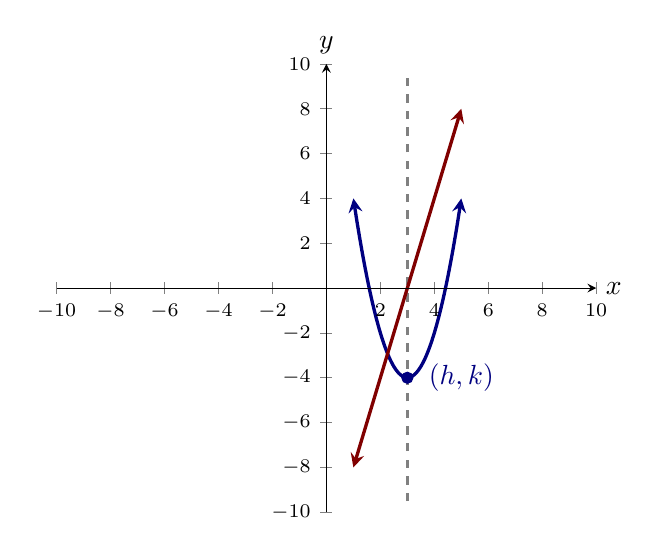
\begin{tikzpicture}
     \begin{axis}[
                domain=-10:10, ymax=10, xmax=10, ymin=-10, xmin=-10,
                axis lines =center, xlabel=$x$, ylabel=$y$,
                ytick={-10,-8,-6,-4,-2,2,4,6,8,10},
                xtick={-10,-8,-6,-4,-2,2,4,6,8,10},
                ticklabel style={font=\scriptsize},
                every axis y label/.style={at=(current axis.above origin),anchor=south},
                every axis x label/.style={at=(current axis.right of origin),anchor=west},
                axis on top,
                ]


        \addplot [draw=penColor, very thick, smooth, domain=(1:5),<->] {2*(x-3)^2 - 4};
        \addplot [line width=1, gray, dashed,samples=100,domain=(-9.5:9.5)] ({3},{x});
        \addplot [color=penColor,only marks,mark=*] coordinates{(3,-4)};
        
        \addplot [draw=penColor2, very thick, smooth, domain=(1:5),<->] {4*(x-3)};

        \node[penColor] at (axis cs:5,-4) {$(h, k)$};
        %\node[penColor] at (axis cs:5,-9) {$-0.5 x^2 - 5 x + 15.5$};



    \end{axis}
\end{tikzpicture}
\end{image}
Our linear rate of change function now informs us about the behavior of $f$. \\



\begin{conclusion}  \textbf{\textcolor{green!50!black}{Behavior}}

$\blacktriangleright$ When the linear rate of change function $iRoC_f(x) < 0$, then $f(x)$ is decreasing. \\

$\blacktriangleright$ When the linear rate of change function $iRoC_f(x) > 0$, then $f(x)$ is increasing. \\

$\blacktriangleright$ When the linear rate of change function $iRoC_f(x) = 0$, then $f(x)$ is neither increasing nor decreasing and the graph of $y = f(x)$ is flat. 

\end{conclusion}


As we can see, the behavior of our function, $f(x)$, can change drastically where $iRoC_f(x) = 0$.  Such domain numbers deserve a special name.



\begin{definition} \textbf{\textcolor{green!50!black}{Critical Number}}  


Let $f$ be a function. Let $x_0$ be a number in the domain of $f$ such that $iRoC_f(x_0) = 0$ or $iRoC_f(x_0)$ does not exist.

Then $x_0$ is called a \textbf{critical number}.


\end{definition}
\textbf{Note: } Domain numbers where $iRoC_f$ doesn't exist are also places where a function's behavior can change drastically.



\begin{procedure} \textbf{\textcolor{blue!75!black}{iRoC for Quadratic Functions}} 



Let $Q$ be a quadratic function.

Then $Q(x) = a (x - h)^2 + k$, for some $a$, $h$, and $k$ with $a \ne 0$. \\

Then, $iRoC_Q(x) = 2 a (x - h)$. \\


\textbf{Procedure:}. It appears that the $2$ in the exponent has slid down in front of the leading coefficient and the constant term $k$ has been removed.



\end{procedure}



We have a procedure for obtaining the $iRoC$ of a quadratic function, when the formula is in vertex form (completed square form). \\

What about standard form? \\



\begin{align*}
Q(x) & = a (x - h)^2 + k \\
     & = a \, x^2 - 2 \, a \, h \, x + a \, h^2 \, k \\
     & = a \, x^2  + (- 2 \, a \, h) x + (a \, h^2 \, k) 
\end{align*}


\begin{align*}
iRoC_Q(x) &= 2 a (x - h) \\
          & = 2 \, a \, x - 2 \, a \, h  \\
\end{align*}





\begin{procedure} \textbf{\textcolor{blue!75!black}{iRoC for Quadratic Functions}} 



Let $Q$ be a quadratic function.

Then $Q(x) = a \, x^2 + b \, x + c$, for some $a$, $b$, and $c$ with $a \ne 0$. \\

Then, $iRoC_Q(x) = 2 \, a \, x + b$. \\


\textbf{Procedure:}. It appears that the $2$ in the exponent has slid down in front of the leading coefficient, the linear coefficent has remained, and the constant term as been removed. 



\end{procedure}

There is probably an overall pattern going on here. \\












\subsection*{Maximums and Minimums}




The maximum and minimum values of a quadratic function, $f$, are visually encoded in the highest and lowest points on the  graph, which is the vertex of the parabola.

Depending on the sign of $a$, the maximum or minimum value of $f(x) = a \, x^2 + b \, x + c$ occurs at $\frac{-b}{2a}$. The maximum or minimum value is $f\left( \frac{-b}{2a} \right)$


Depending on the sign of $a$, the maximum or minimum value of $f(x) = a \, (x - h)^2 + k$ is $k$ and occurs at $h = \frac{-b}{2a}$. 







We can also look at the linear $iRoC_f(x)$ function.  Where $iRoC_f(x) = 0$ is where the vertex is located, which encodes the maximum or minimum value of $f$.





\begin{align*}
iRoC_Q(x)       &= 0  \\
2 \, a \, x + b  & = 0  \\
x     &=  \frac{-b}{2a}
\end{align*}




\textbf{\textcolor{blue!55!black}{$\blacktriangleright$}}  $\frac{-b}{2a}$ is the critical number for a quadratic function given in standard form: $a \, x^2 + b \, x + c$.



\textbf{\textcolor{blue!55!black}{$\blacktriangleright$}}  $h$ is the critical number for a quadratic function given in vertex form: $a \, (x - h)^2 + c$.



\textbf{\textcolor{blue!55!black}{$\blacktriangleright$}}  $\frac{r_1 + r_2}{2}$ is the critical number for a quadratic function given in factored form: $a \, (x - r_1) (x - r_2)$.

















\subsection*{Range}

$\blacktriangleright$  \textbf{Vertex Form} \\

The graph of a quadratic function is a parabola, which is easily connected to the completed square form of the formula.

Below is the graph of $y = f(x) = a (x - h)^2 + k$, with $a$, and $h$, and $k$ all real numbers and $a > 0$. The extreme point is called the \textbf{vertex}. If $a<0$, then the parabola would have opened downward and the extreme point would be at the top.

\begin{image}
\begin{tikzpicture}
     \begin{axis}[
                domain=-10:10, ymax=10, xmax=10, ymin=-10, xmin=-10,
                axis lines =center, xlabel=$x$, ylabel=$y$,
                ytick={-10,-8,-6,-4,-2,2,4,6,8,10},
                xtick={-10,-8,-6,-4,-2,2,4,6,8,10},
                ticklabel style={font=\scriptsize},
                every axis y label/.style={at=(current axis.above origin),anchor=south},
                every axis x label/.style={at=(current axis.right of origin),anchor=west},
                axis on top,
                ]


        \addplot [draw=penColor, very thick, smooth, domain=(1:5),<->] {2*(x-3)^2 - 4};
        \addplot [line width=1, gray, dashed,samples=100,domain=(-9.5:9.5)] ({3},{x});
        \addplot [color=penColor2,only marks,mark=*] coordinates{(3,-4)};
        


        \node[penColor] at (axis cs:5,-4) {$(h, k)$};
        %\node[penColor] at (axis cs:5,-9) {$-0.5 x^2 - 5 x + 15.5$};



    \end{axis}
\end{tikzpicture}
\end{image}

The vertex visually encodes the  minimum (or maximum) value of the function. 




If $a<0$, then everything is reveresed.







\begin{image}
\begin{tikzpicture}
     \begin{axis}[
                domain=-10:10, ymax=10, xmax=10, ymin=-10, xmin=-10,
                axis lines =center, xlabel=$x$, ylabel=$y$, 
                ytick={-10,-8,-6,-4,-2,2,4,6,8,10},
                xtick={-10,-8,-6,-4,-2,2,4,6,8,10},
                ticklabel style={font=\scriptsize},
                every axis y label/.style={at=(current axis.above origin),anchor=south},
                every axis x label/.style={at=(current axis.right of origin),anchor=west},
                axis on top,
                ]


        \addplot [draw=penColor, very thick, smooth, domain=(1:5),<->] {-2*(x-3)^2 + 4};
        \addplot [line width=1, gray, dashed,samples=100,domain=(-9.5:9.5)] ({3},{x});
        \addplot [color=penColor2,only marks,mark=*] coordinates{(3,4)};
        


        \node[penColor] at (axis cs:5,4) {$(h, k)$};
        %\node[penColor] at (axis cs:5,-9) {$-0.5 x^2 - 5 x + 15.5$};



    \end{axis}
\end{tikzpicture}
\end{image}











We can see from the formula $f(x) = a (x - h)^2 + k$, that since $(x - h)$ is squared, and thus nonnegative, the range of $f$ depends on the sign of $a$. \\

When $a>0$, the values of $f(x)$ are greater than or equal to $k$. This corresponds to the graph opening up.  The only way to get the least value possible for $f$ is to select $x = h$. That corresponds to the vertex $(k, h)$. \\



When $a<0$, the values of $f(x)$ are less than or equal to $k$. This corresponds to the graph opening down.  The only way to get the greatest value possible for $f$ is to select $x = h$. That corresponds to the vertex $(k, h)$.  \\

We can see that the implied range of a quadratic comes in two types.  

\begin{itemize}
\item The range could be all real numbers greater than or equal to some particular number:  $\{ r \in \textbf{R} \, | \, r \geq k \}$.
\item The range could be all real numbers less than or equal to some particular number:  $\{ r \in \textbf{R} \, | \, r \leq k \}$.
\end{itemize}

If there is a stated domain, then the range will be restricted appropriately. \\










\begin{center}
\textbf{\textcolor{green!50!black}{ooooo=-=-=-=-=-=-=-=-=-=-=-=-=ooOoo=-=-=-=-=-=-=-=-=-=-=-=-=ooooo}} \\

more examples can be found by following this link\\ \link[More Examples of Quadratic Behavior]{https://ximera.osu.edu/csccmathematics/precalculus1/precalculus1/quadraticBehavior/examples/exampleList}

\end{center}




\end{document}




